\section{Część radiowa}

% Do wykonania przetwarzania w części radiowej wykorzystaliśmy radio

Radio które posiadaliśmy w laboratorium USRP-2932 niestety nie nadaje się do odbioru sygnału APRS ze względu na dolną granicę pasma 400 MHz. Zamiast tego wykorzystaliśmy je do odbioru transmisji o modulacji LoRa wykorzystując jako nadajnik układ z poprzedniego projektu: Orange Pi połączony z układem nadawczym. Do testów transmisji APRS wykorzystaliśmy inne radio programowalne.

Dodatkowo jeden z członków podjął się wykonania części odbiornika (samej demodulacji) na układzie FPGA z przetwornikiem analogowo-cyfrowym. Niestety nie możemy wykorzystać tego rozwiązania, ponieważ brakuje synchronizacji i części analogowej (filtry, mieszacz).

\begin{figure}[!htbp]
 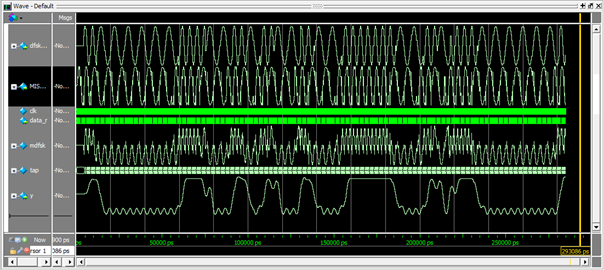
\includegraphics[width=0.8\textwidth]{symulacja}
 \centering
 \caption{Wynik symulacji demodulacji APRS na FPGA}
\end{figure}

Okazało się, że gotowe projekty oprogramowania demodulatora zarówno APRS jak i LoRa są dostępne w internecie z otwartym oprogramowaniem w GNU radio, więc wystarczyło je przetestować w naszych układach.
